\documentclass[conference]{IEEEtran}
\usepackage{cite}
\usepackage{amsmath,amssymb,amsfonts}
\usepackage{algorithmic}
\usepackage{graphicx}
\usepackage{textcomp}
\usepackage{xcolor}
\usepackage[colorlinks,linkcolor=blue]{hyperref}
\def\BibTeX{{\rm B\kern-.05em{\sc i\kern-.025em b}\kern-.08em
    T\kern-.1667em\lower.7ex\hbox{E}\kern-.125emX}}
\begin{document}

\title{Homework for Artificial Intelligence \\ Problem Solving and Practice \\
{\normalsize \vspace{1em} Author: Kailing Wang(\href{mailto:wangkailing151@gmail.com}{Email}) \\ Shanghai Jiao Tong University \\ 2022.6.15}
}

\maketitle

\begin{abstract}
In this homework, I used different self-written unsupervised clustering methods and compared them each to decide which works better to do clustering on the given four datasets.
\end{abstract}

\begin{IEEEkeywords}
Clustering, Dimension Reduction, K-means, Expectation Maximization, Gaussian Mixture Model, Davis-Bouldin Index, Dunn Index, Multiple Dimensional Scaling, Primary Component Analysis, K Nearest Neighborhood, Isometric Mapping
\end{IEEEkeywords}

\section{\textbf{Algorithm and Code}}
I've realized a package-like python script file with name Lo\_clustering\_with\_dr.py, which is now open source on github at \href{https://github.com/Loping151/openFiles/tree/main/2022Spring/AIHomework}{openFiles}. \textbf{I don't think it necessary to explain the algorithm in detail(for that's just copying from book)}, but here I have to explain the specific feature of my code, and special method used during coding. My code is 100\% original, with 0\% copied or online reference. It may not be perfect, but it contains my weeks of hard work.

I realized class KMeans, Gaussian Mixture, Clustering Assessment, MDS, PCA and Isomap along with other tool functions. All the derivation process are from book Machine Learning[\ref{b1}]. I wrote very detailed explanation and usage example in the code file.

\subsection{\textbf{Tool functions}}
\subsubsection{Distance measurement}
Default distances used are Euclidean Distance in the form of function \ref{ED}

\small
\begin{equation}
	d_{ed}(x, y)=\sqrt{\left(x_{1}-y_{1}\right)^{2}+\left(x_{2}-y_{2}\right)^{2}+\cdots+\left(x_{n}-y_{n}\right)^{2}}
	\label{ED}
\end{equation}
\normalsize

Of course, when computing, the square root is unnecessary when we only need to compare, so I wrote square root as an option and defined default cmp function.

I also realized Minkowski Distance \ref{MD}

\begin{equation}
	d_{mk}(x, y)=\sqrt{\sum_{u=1}^{n}{\left|x_u-y_u\right|}}
		\label{MD}
\end{equation}

Users can select p for Minkowski and use it as the distance inside KMeans or Dimension Reduction.

\subsubsection{\textbf{Probability}}
Standard gaussian function \ref{gaussianf} is realized, and the function support vector-like input.

\begin{equation}
	p(\boldsymbol{x})=\frac{1}{(2 \pi)^{\frac{n}{2}}|\boldsymbol{\Sigma}|^{\frac{1}{2}}} e^{-\frac{1}{2}(\boldsymbol{x}-\boldsymbol{\mu})^{\mathrm{T}} \boldsymbol{\Sigma}^{-1}(\boldsymbol{x}-\boldsymbol{\mu})}
	\label{gaussianf}
\end{equation}

\subsubsection{\textbf{Assessment}}
The assessment methods are Davis-Bouldin Index \ref{DBI} (the lower, the better) and Dunn Index \ref{DI} (the higher, the better)

\begin{equation}
	\mathrm{avg}\left(C\right) = \frac{2}{ \left|C\right| \left(\left|C\right|-1\right)}\sum_{1\leqslant i\leq j \leqslant \left|C\right|}\mathrm{dist}\left(x_i, x_j\right)
\end{equation}
\vspace{-0.75em}
\begin{equation}
	\mathrm{diam}\left(C\right) = max_{1\leqslant i\leq j \leqslant \left|C\right|}\mathrm{dist}\left(x_i, x_j\right)
\end{equation}
\vspace{-1em}
\begin{equation}
	d_{min}\left(C_i, C_j\right) = min_{x_i \in C_i, x_j \in C_j}\mathrm{dist}\left(x_i, x_j\right)
\end{equation}
\vspace{-1em}
\begin{equation}
	d_{cen}\left(C_i, C_j\right) = \mathrm{dist}\left(\mu_i, \mu_j\right)
\end{equation}
\begin{equation}
	\mathrm{DBI}=\frac{1}{k} \sum_{i=1}^{k} \max _{j \neq i}\left(\frac{\operatorname{avg}\left(C_{i}\right)+\operatorname{avg}\left(C_{j}\right)}{d_{\text {cen }}\left(C_{i}, C_{j}\right)}\right)
	\label{DBI}
\end{equation}
\begin{equation}
	\mathrm{DI}=\min _{1 \leqslant i \leqslant k}\left\{\min _{j \neq i}\left(\frac{d_{\min }\left(C_{i}, C_{j}\right)}{\max _{1 \leqslant l \leqslant k} \operatorname{diam}\left(C_{l}\right)}\right)\right\}
\label{DI}
\end{equation}

Both indexes are internal, for there isn't a standard for this homework.

\subsubsection{\textbf{Other}}
Some of the functions for vectors are realized, for I didn't know we could use numpy. Vector add and decide and vector.T.vector were realized. Other tools include data normalize, dijkstra.

\subsection{\textbf{Clustering}}
\subsubsection{\textbf{KMeans}}
My KMeans allows user to decide initialization seed or directly give the initial centroids. The parameter tolerance is to stop the iteration when the maximum movement of the centroid is lower than tol, and the parameter stop means maximum iteration round.

My KMeans finds initial centroids by Gaussian fit each dimension of the dataset and randomly choose a value within range $[\mu-\sigma, \mu+\sigma)$ as the coordinate of this dimension for one centroid. This method is not as good as KMeans++, but it is original.

After comparing, my KMeans works as fine as the one in sklearn under most tested seeds. As I can decide the initial centroid and support any distance function, my KMeans sometimes work better. In this home work, my KMeans converges after only 1 rounds for problem 1 and 4 rounds for problem 2.

\subsubsection{\textbf{GMM}}
It's really hard to code such complex matrix calculation as a new numpy learner, so the code is a bit ugly. My GMM include all the features of KMeans. As for initialization, random initialize sometimes work badly. I recommend using the default method: initialize with KMeans to get clusters, and then calculate mean position and covariance matrix.

The update formulas are as follows \ref{gmmf1}, \ref{gmmf2}:

 \begin{equation}
 	\begin{aligned}
 		p_{\mathcal{M}}\left(z_{j}=i \mid \boldsymbol{x}_{j}\right) &=\frac{P\left(z_{j}=i\right) \cdot p_{\mathcal{M}}\left(\boldsymbol{x}_{j} \mid 	z_{j}=i\right)}{p_{\mathcal{M}}\left(\boldsymbol{x}_{j}\right)} \\
 		&=\frac{\alpha_{i} \cdot p\left(\boldsymbol{x}_{j} \mid \boldsymbol{\mu}_{i}, \boldsymbol{\Sigma}_{i}\right)}{\sum_{l=1}^{k} \alpha_{l} \cdot p\left(\boldsymbol{x}_{j} \mid \boldsymbol{\mu}_{l}, \boldsymbol{\Sigma}_{l}\right)}
 	\label{gmmf1}
 	\end{aligned}
 \end{equation}

 \begin{equation}
 	\begin{aligned}
 		&\boldsymbol{\mu}_{i}^{\prime}=\frac{\sum_{j=1}^{m} \gamma_{j i} \boldsymbol{x}_{j}}{\sum_{j=1}^{m} \gamma_{j i}} \\
 		&\boldsymbol{\Sigma}_{i}^{\prime}=\frac{\sum_{j=1}^{m} \gamma_{j i}\left(\boldsymbol{x}_{j}-\boldsymbol{\mu}_{i}^{\prime}\right)\left(\boldsymbol{x}_{j}-\boldsymbol{\mu}_{i}^{\prime}\right)^{\mathrm{T}}}{\sum_{j=1}^{m} \gamma_{j i}} \\
 		&\alpha_{i}^{\prime}=\frac{\sum_{j=1}^{m} \gamma_{j i}}{m}
 	\end{aligned}
 	\label{gmmf2}
 \end{equation}

It usually converge after more but less than 150 rounds in less than 1 minute.

\subsection{\textbf{Dimensional Reduction}}
\subsubsection{\textbf{MDS}}
Multiple Dimensional Scaling, easy to realize with numpy.linalg, could convert data of any dimension to certain dimension fast.
\subsubsection{\textbf{PCA}}
Primary Component Analysis. Similar to MDS, use bigger eigenvalues and vectors to reduce dimension.
\subsubsection{\textbf{Isomap}}
Calculate distance with dijkstra on a connected graph generated by KNN, and then user can shoose MDS or PCA to reduce dimension.

The former two method runs rather fast, but because dijkstra is slow and k need to be large in KNN inside Isomap for sometimes data is not very sparse, Isomap usually takes a while.


\section{\textbf{Problem 1}}
The distribution of dataset 1 is shown in Fig. \ref{p1raw}. and the problem is to divide it into to clusters.

There is no obvious boundary. So it's actually hard to decide how to do clustering.

\begin{figure}[htbp]
	\centerline{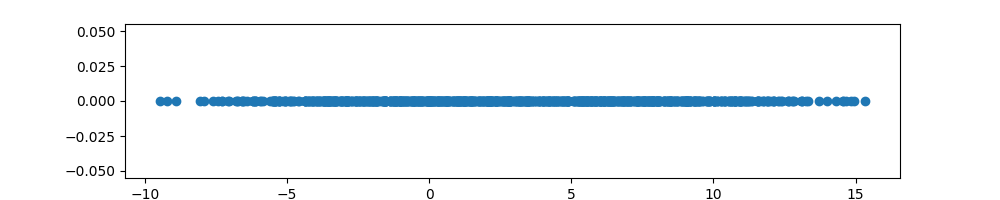
\includegraphics[scale=0.375]{p1raw.png}}
	\caption{Distribution of dataset 1}
	\label{p1raw}
\end{figure}

\subsection{Method 1: Simple average}
Suggest it is a simple linearly separable problem, and the distribution then we just need to calculate the mean or median of the dataset. I chose to devide by mean, and the result is Fig. \ref{m1p1}.

\begin{figure}[htbp]
	\centerline{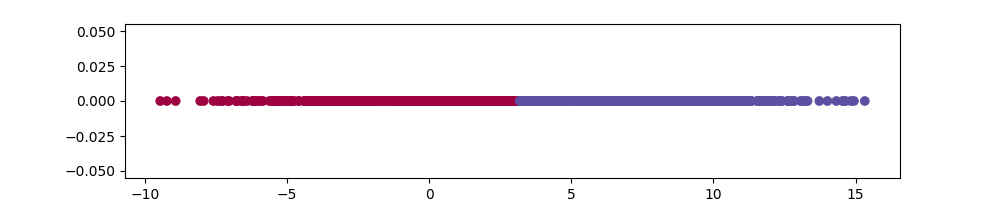
\includegraphics[scale=0.375]{m1p1.png}}
	\caption{Clustering using method 1 on dataset 1}
	\label{m1p1}
\end{figure}

\subsection{Method 2: KMeans}
I tried KMeans myself, and the result is like Fig. \ref{m2p1}. Actually the result looks just like dividing by mean valve.

\begin{figure}[htbp]
	\centerline{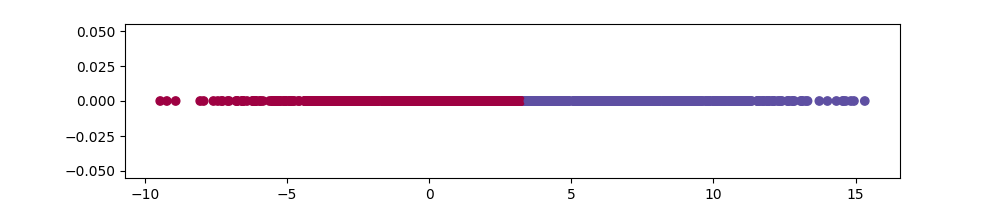
\includegraphics[scale=0.375]{m2p1.png}}
	\caption{Clustering using method 2 on dataset 1}
	\label{m2p1}
\end{figure}

\subsection{Method 3: Kernel function+KMeans}
Anyway, the dataset doesn't seem to be separable at all. However, since no feature is known, I have no way to design a kernel function, so
I look into the distance between points, and found that the points on both ends seem to part farther from points in the middle area. I draw Fig. \ref{distance1}. to describe this feature, based on which I designed function \ref{kernel1}:

\begin{figure}[htbp]
	\centerline{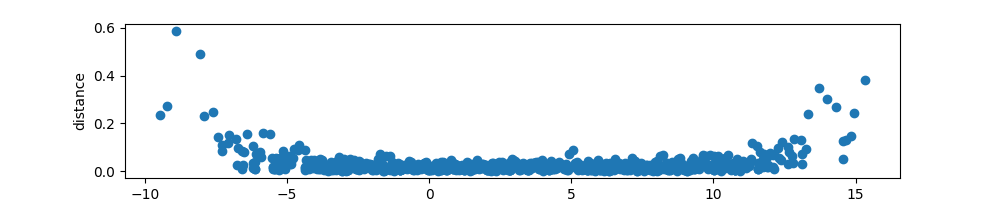
\includegraphics[scale=0.375]{distance1.png}}
	\caption{Distance between a point and its neighbors}
	\label{distance1}
\end{figure}

\begin{equation}
	f(x) = -\left(x-r\right)^4
	\label{kernel1}
\end{equation}
where $r$ is the radius of data defined as \ref{kernel2}

\begin{equation}
	r = x_{max} - x_{min} \quad for \quad x \in data
	\label{kernel2}
\end{equation}

Fig. \ref{m3p1}. shows the result.


\begin{figure}[htbp]
	\centerline{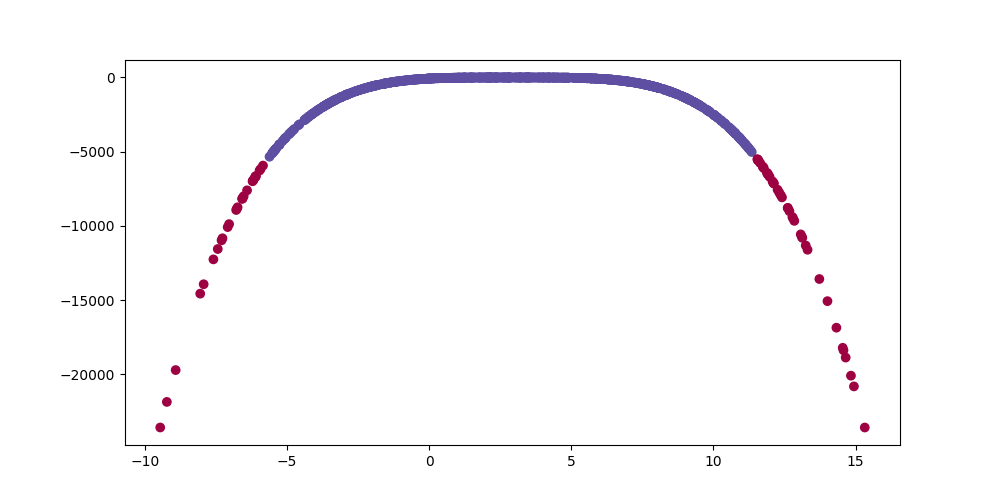
\includegraphics[scale=0.35]{m3p1.png}}
	\caption{Clustering using method 3 on dataset 1}
	\label{m3p1}
\end{figure}

It seems that I've perfectly separates points on both ends from the central ones.
\subsection{Method 4: Expectation Maximization(GMM)}
I tried to draw dataset 1 with a histogram Fig. \ref{his}

\begin{figure}[htbp]
	\centerline{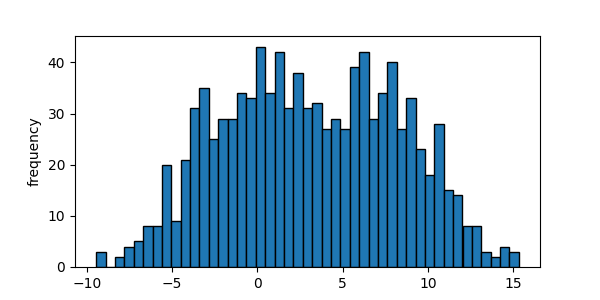
\includegraphics[scale=0.6]{his.png}}
	\caption{Histogram of dataset 1}
	\label{his}
\end{figure}

This figure reminds me of Gaussian Distribution. So I realized GMM and tried. See Fig \ref{m4p1gaussian}, in which I also plotted gaussian probability
\begin{figure}[htbp]
	\centerline{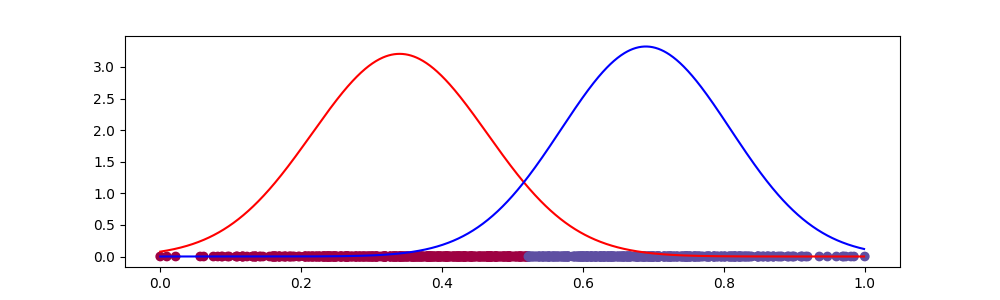
\includegraphics[scale=0.375]{m4p1gaussian.png}}
	\caption{Method 4 on dataset 1 and gaussian}
	\label{m4p1gaussian}
\end{figure}

Here KMeans converged after 1 round, and GMM 23 rounds. I chose this as the final result.
\section{\textbf{Problem 2}}
The dataset is like Fig. \ref{p2raw}.

\begin{figure}[htbp]
	\centerline{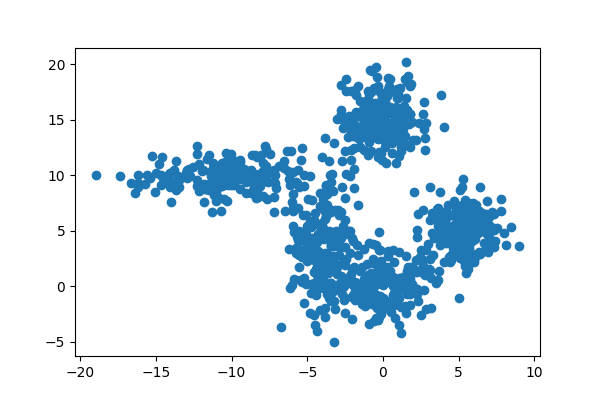
\includegraphics[scale=0.5]{p2raw.png}}
	\caption{Distribution of dataset 2}
	\label{p2raw}
\end{figure}

Obviously we can recognize four or five clusters.

\subsection{The best K(Clusters for KMeans)}
Fig \ref{p2_345} shows results using KMeans for cluster number from 3 to 6.

\begin{figure}[h]
	\centering
	{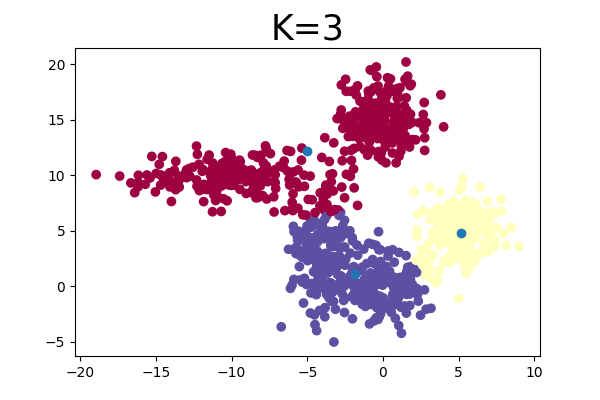
\includegraphics[scale=0.28]{k=3}}
	{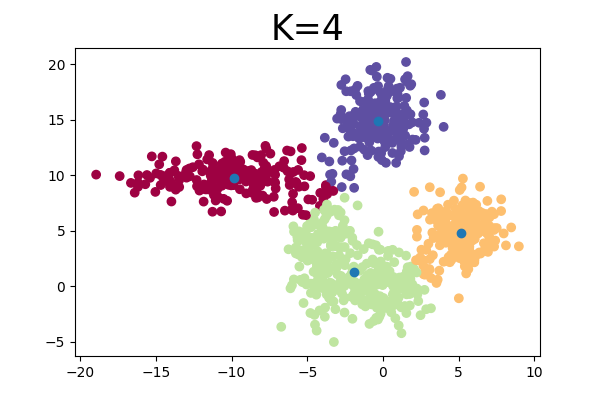
\includegraphics[scale=0.28]{k=4}}
	{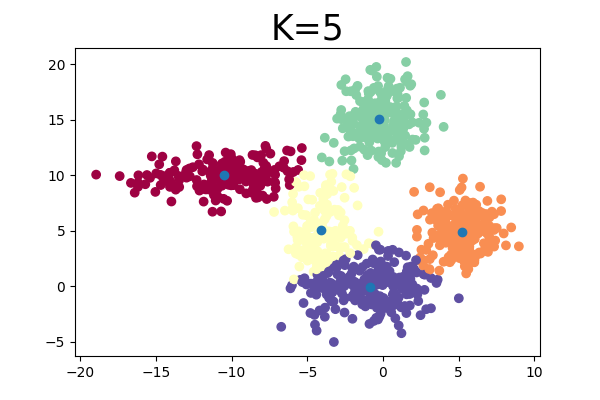
\includegraphics[scale=0.28]{k=5}}
	{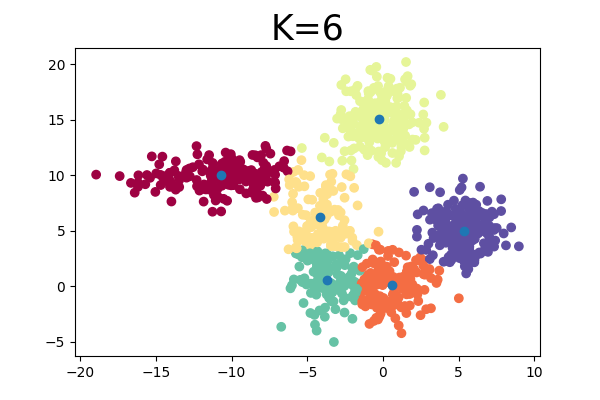
\includegraphics[scale=0.28]{k=6}}
	\caption{K = 3, 4, 5, 6 on dataset 2}
	\label{p2_345}
\end{figure}

To further decide the best K for KMeans, I calculate DBI and DunnI for K from 2 to 10, as shown in Fig. \ref{DDI}.

Both index decide that 4 cluster is the best choice.

\begin{figure}[htbp]
	{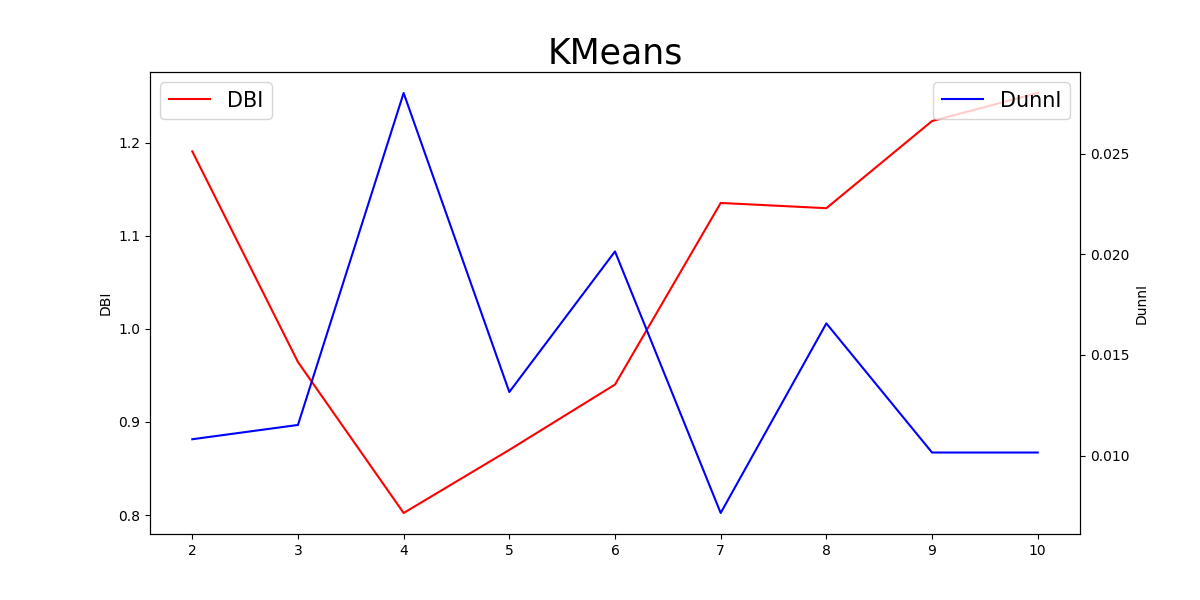
\includegraphics[scale=0.3]{KM_DDI.png}}
	{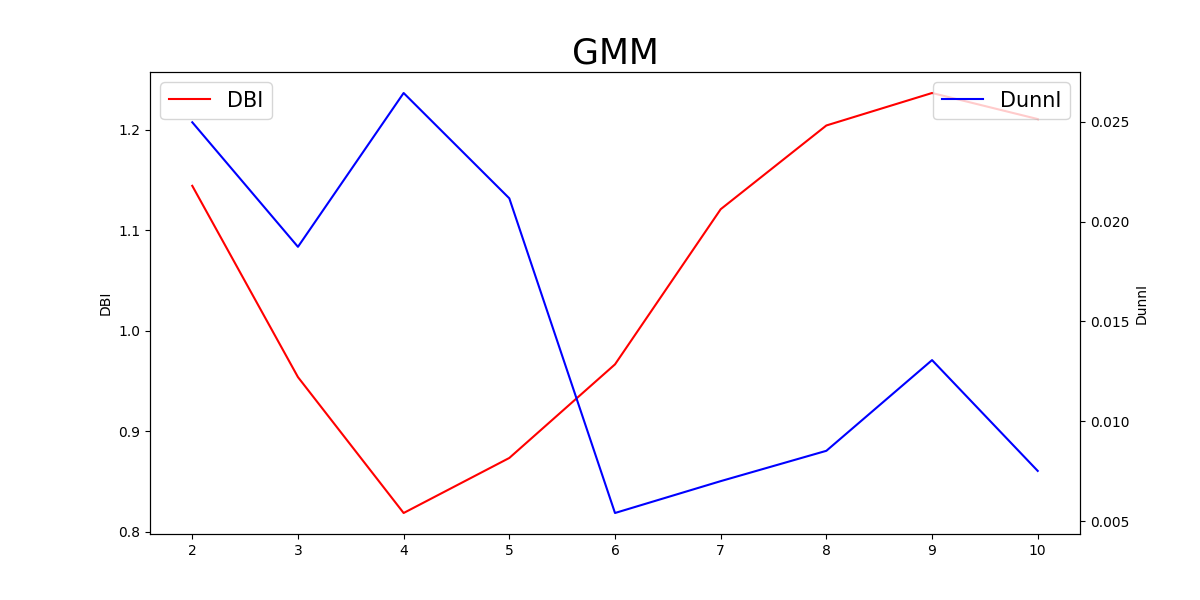
\includegraphics[scale=0.3]{GM_DDI.png}}
	\caption{DBI and DI for KMeans and GMM on dataset 2}
	\label{DDI}
\end{figure}

\subsection{The best C(components for GMM)}
I repeated this process using GMM, and the index (in Fig. \ref{DDI}.) also shows C should be 4.

Fig. \ref{KG_cmp}. compares the results of the two. As we can see, the boundaries of KMeans are strict lines, and looks curt, while those of GMM looks more smooth. Actually when C = 5 the result looks really beautiful(all the pictures are attached with code file). I feel pity 5 is not the best.

\begin{figure}[htbp]
	{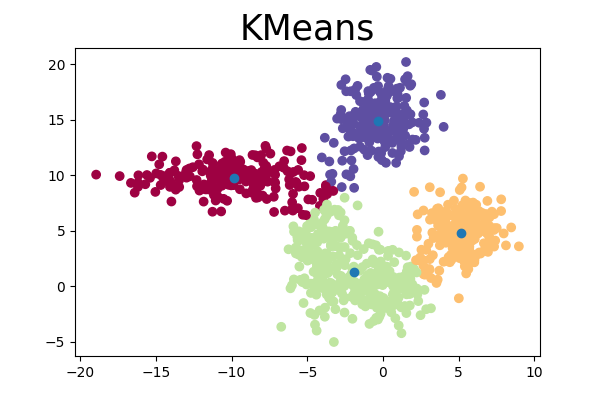
\includegraphics[scale=0.28]{m1p2.png}}
	{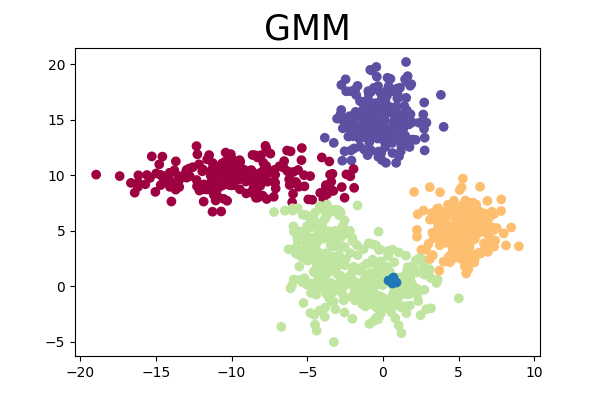
\includegraphics[scale=0.28]{m2p2.png}}
	\caption{Results from KMeans and GMM on dataset 2}
	\label{KG_cmp}
\end{figure}

After thinking twice, I decide to put Fig. \ref{pity}. here. I suppose the TA generated 5 clusters, but the data was just not very well that the index showed 4 is better. Anyway, I have to choose 4 cluster with GMM as the final result.

\begin{figure}[htbp]
	\centerline{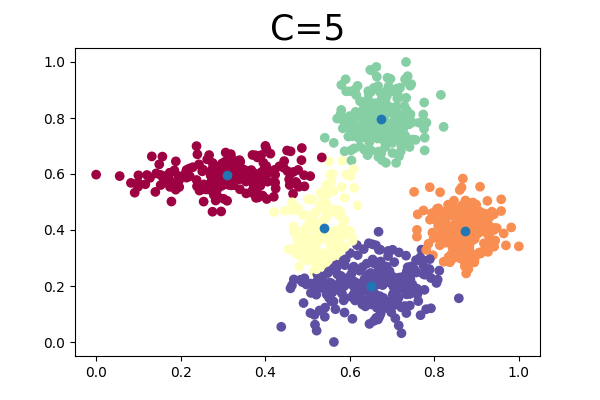
\includegraphics[scale=0.5]{g=5.png}}
	\caption{GMM C=5 on dataset 2}
	\label{pity}
\end{figure}

\section{\textbf{Problem 3}}
\subsection{Dimension Reduction}
	Fig. \ref{MDS_PCA1}. is the result of MDS and PCA reducing dataset 3 to 2 dimension. One of the clusters is obvious, but the other two are close.

\begin{figure}[htbp]
	{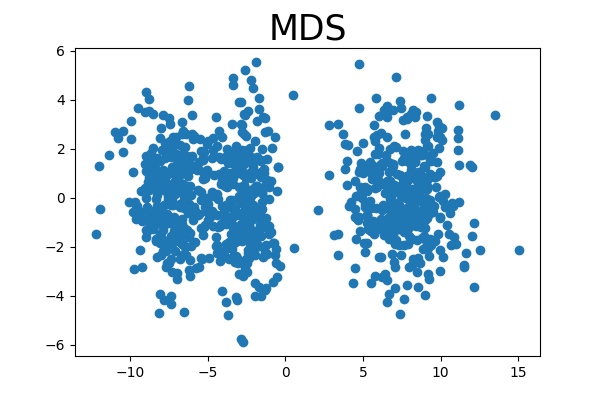
\includegraphics[scale=0.28]{p3MDS.png}}
	{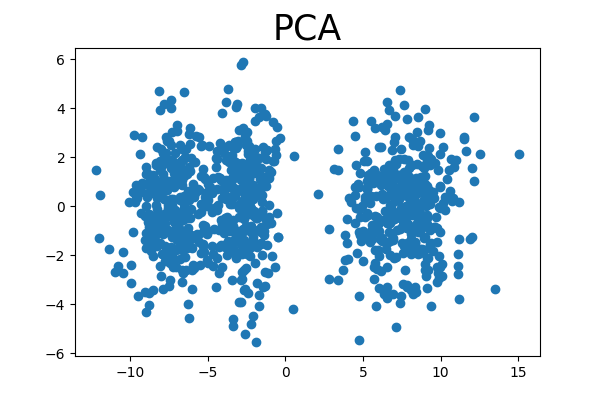
\includegraphics[scale=0.28]{p3PCA.png}}
	\caption{Results of MDS and PCA on dataset 3}
	\label{MDS_PCA1}
\end{figure}

\subsection{Clustering}
I tried to use different combination of method do clustering. Some one said in the QQ chat group that he directly applied KMeans without dimensional reduction, so I made a simple comparison. I tried MDS+KMeans, MDS+GMM, PCA+KMeans, PCA+GMM, KMeans-only and GMM-only. I won't put all the graph here, for there are already too much graphs.

Fig. \ref{DRCMP}. shows result of MDS+KMeans and KMeans-only. They are likely the same. So what's the point in dimension reduction? I can't understand. The dataset wasn't properly constructed.

\begin{figure}[htbp]
	{\includegraphics[scale=0.28]{P3MK2.png}}
	{\includegraphics[scale=0.28]{p3K.png}}
	\caption{MDS+KMeans and KMeans-only on dataset 3}
	\label{DRCMP}
\end{figure}

But I'm not satisfied. there are two clusters very close. I wonder if some of the distance was ignored during reduction. Then I tried to reduce the data to 5 dimension and apply GMM, and find Fig. \ref{P3MG5}.

\begin{figure}[htbp]
	\centerline{\includegraphics[scale=0.5]{P3MG5.png}}
	\caption{Results of MDS and PCA on dataset 3}
	\label{P3MG5}
\end{figure}

\subsection{Final solution}
I tried to apply Isomap to reduce dimension, but I find that the k in KNN used in Isomap need to be over 200 to get the k-distance graph connected, which means there must be a huge gap between the data, and the data is not sparse at all! So I gave up coding Kernelized PCA.

I thought of a method: I could only apply Isomap only on the closer two clusters. I used KMeans to separate the obvious cluster, and then use Isomap to reduce dimension of the other part of the dataset. However, the result was like Fig. \ref{P3IsoR}. There must be something in the higher dimension, but I can't figure out a way to visualize it. At last, I used PCA to reduce the data to 5 dimension and then apply Isomap. Then I use KMeans to do clustering. The result is as Fig. \ref{P3IsoK}

\begin{figure}[htbp]
	\centerline{\includegraphics[scale=0.5]{P3IsoR.png}}
	\caption{Isomap on dataset 3}
	\label{P3IsoR}
\end{figure}

\begin{figure}[htbp]
	\centerline{\includegraphics[scale=0.5]{P3IsoK.png}}
	\caption{PCA-Isomap and KMeans on dataset 3}
	\label{P3IsoK}
\end{figure}

In fact, I simply cut the reduced-to 2 dataset 3 with line x = 1. I chose k=10 for KNN in Isomap. The final result is Fig. \ref{P3FIN}. and the final label is Fig. \ref{P3FIN}.

\begin{figure}[htbp]
	\includegraphics[scale=0.28]{P3Fin.png}
	\includegraphics[scale=0.28]{P3Fin3.png}
	\caption{Final result on dataset 3}
	\label{P3FIN}
\end{figure}

\section{\textbf{Problem 4}}
This problem is nothing more than the combination of problem 2 and problem 3. Fig. \ref{P4RAW}. shows reducing dimension of dataset 4 using MDS and PCA. 2000 points was chosen to plot to look clearer. Under a dataset of 10000, MDS takes much longer for it concerns distance calculation. Isomap includes dijkstra, so it needs around a week to finish calculation because for dijkstra is $O(n^3)$.

\begin{figure}[htbp]
	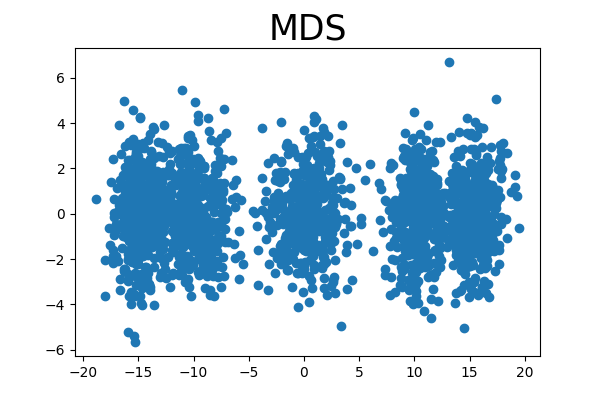
\includegraphics[scale=0.28]{P4RM.png}
	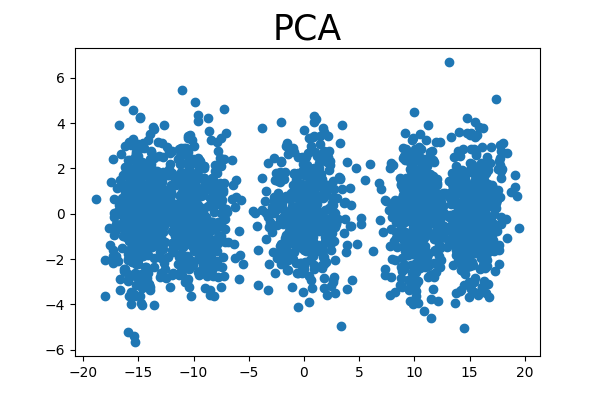
\includegraphics[scale=0.28]{P4RP.png}
	\caption{Dimension reduction on dataset 4}
	\label{P4RAW}
\end{figure}

During plotting, I realized the result from MDS and PCA are completely the same, and I also find all the other 127 dimension are useless. The deciding factor is the first dimension only. Anyway, I still calculated DBI and DunnI for k form 2 to 10. PCA was faster, so I used PCA to reduce the dataset to dimension 3, 5 and 10 and applied KMeans and GMM. This time, DBI was lowest at 2, and DunnI highest at 3. However, at least 5 obvious clusters are recognized.

\begin{figure}[htbp]
	\centerline{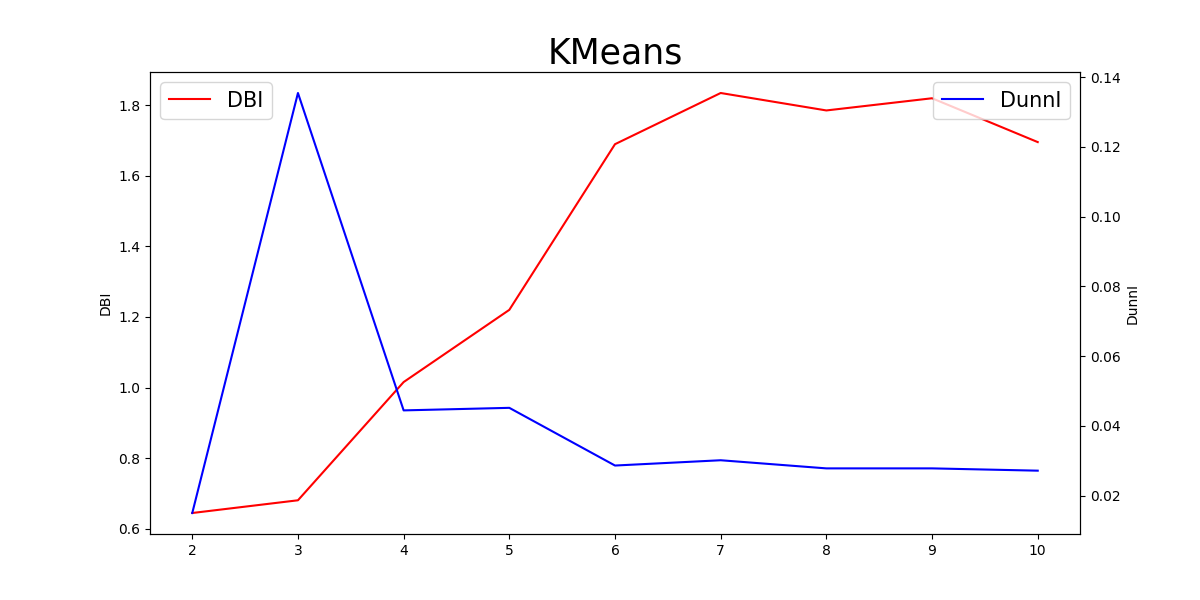
\includegraphics[scale=0.3]{KM_DDI4.png}}
	\centerline{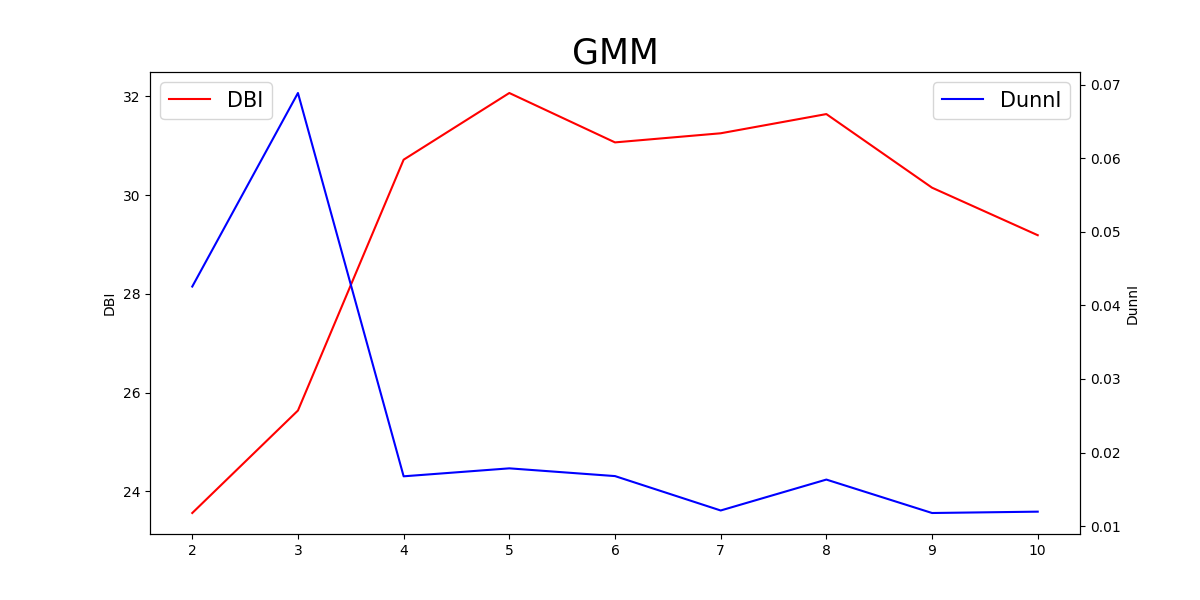
\includegraphics[scale=0.3]{GM_DDI4.png}}
	\caption{DBI and DI on dataset 4(reduced to 5)}
	\label{KMDDI4}
\end{figure}

I also have to show you the result of GMM(C=10) Fig. \ref{GMM10}. It's absurd, but beautiful.

\begin{figure}[htbp]
	\centerline{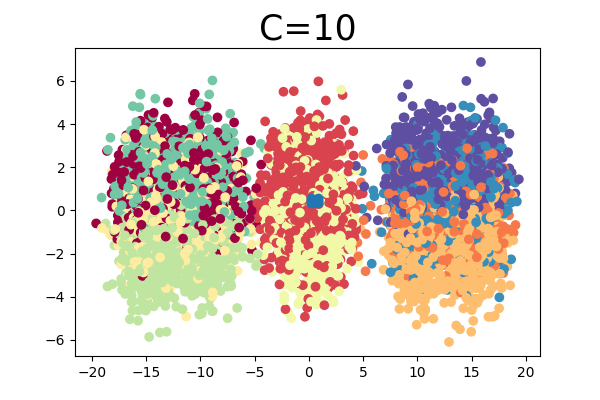
\includegraphics[scale=0.5]{4g=10.png}}
	\caption{PCA and GMM(C=10) on dataset 4}
	\label{GMM10}
\end{figure}

Next I tried directly apply KMeans directly, and the index and results are about the same of PCA and KMeans. This also provide evidence for the dataset is poorly constructed.

I tried and tried, but I can hardly give a reason for choosing k = 5. Square error was considered, but the elbow is ambiguous to determine.

Finally, I choose PCA(to 3) and KMeans(k = 5) to give the final label Fig. \ref{P4FIN}

\begin{figure}[htbp]
	\centerline{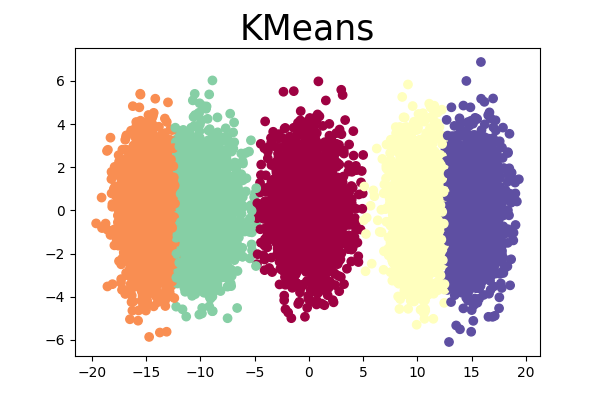
\includegraphics[scale=0.5]{p4Fin.png}}
	\caption{Final result on dataset 4}
	\label{P4FIN}
\end{figure}

\section*{Acknowledgment}
Here I sincerely thank Professor Cewu Lu and Lixin Yang and other TA, who open the door of machine learning and deep learning for me.

\begin{thebibliography}{00}
\bibitem{b1} \href{https://books.google.com/books/about/%E6%9C%BA%E5%99%A8%E5%AD%A6%E4%B9%A0.html?id=j0G8nQAACAAJ}{Machine Learning.} Zhou Zhihua. Tsinghua University Press. 2016. \label{b1}
\end{thebibliography}
\end{document}
